%!TEX root = origin.TEX
\chapter{Marco teórico}
\pagenumbering{arabic}
\setcounter{page}{15}
\renewcommand{\baselinestretch}{2} %doble espacio paratodo el texto

En este capítulo se presenta una reseña del material bibliográfico investigado con relación a los temas considerados en esta investigación. Los conocimientos investigados son muy amplios, principalmente aquel que ayudó a consolidar las bases del conocimiento científico para elaborar esta tesis, como lo son los temas de optimización combinatoria, complejidad computacional, metaheurísticas, ciencia de la información y logística, conocimientos sin los cuales sería difícil de modelar y solucionar matemática y computacionalmente cualquier tipo de problema de optimización.

\section{Aprendizaje Profundo} 
	En los primeros días de la inteligencia artificial, el campo atacó y resolvió rápidamente problemas que son intelectualmente difíciles para los seres humanos pero relativamente sencillos para las computadoras, problemas que pueden describirse mediante una lista de reglas formales y matemáticas. El verdadero desafío para la inteligencia artificial fue y es resolver las tareas que son fáciles de realizar para las personas pero difíciles de describir de manera formal, problemas que resolvemos intuitivamente, que se sienten automáticos, como reconocer palabras, rostros u objetos en las imágenes \citep{Goodfellow-et-al-2016}.

	\vskip 0.4cm  
	Si bien aprendizaje automático(del inglés, {\bf machine learning}) se describe a menudo como una subdisciplina de la inteligencia artificial(IA), es mejor considerarla como la mejor técnica de la disciplina; es decir, es el campo de la IA que hoy en día muestra la mayor promesa al proporcionar herramientas que la industria y la sociedad pueden usar para producir algún cambio. En tal sentido,el aprendizaje automático toma algunas de las ideas centrales de la inteligencia artificial y las enfoca en resolver problemas del mundo real con redes neuronales diseñadas para imitar nuestra propia toma de decisiones; sin embargo, el aprendizaje profundo o avanzado de máquinas (del inglés, {\bf deep learning}) se centra aún más estrechamente en un subconjunto de herramientas y técnicas del aprendizaje automático y los aplica a la solución de casi cualquier problema que requiera "pensamiento", ya sea humano o artificial.

	\vskip 0.4cm  
	El aprendizaje profundo es un enfoque específico utilizado para construir y entrenar redes neuronales para la toma de decisiones altamente prometedoras. Se considera que un algoritmo es profundo si los datos de entrada se pasan a través de una serie de no linealidades o transformaciones no lineales antes de que se emita. Este enfoque permitir que las computadoras aprendan de la experiencia y entiendan el mundo en términos de una jerarquía de conceptos, con cada concepto definido a través de su relación con conceptos más simples. Al reunir el conocimiento de la experiencia, este enfoque evita la necesidad de que los operadores humanos especifiquen formalmente todo el conocimiento que necesita la computadora. La jerarquía de conceptos permite que la computadora aprenda conceptos complicados mediante la construcción de los más simples. Si dibujamos un gráfico que muestra cómo estos conceptos se construyen uno encima del otro, el gráfico es profundo, con muchas capas. Por esta razón, este enfoque se conoce como el aprendizaje profundo de la inteligencia artificial \citep{Goodfellow-et-al-2016}.

	\vskip 0.4cm 
	El aprendizaje profundo elimina el hecho que se tenga que realizar una identificación manual de las características en los datos y, en cambio, depende del proceso de capacitación que tenga para descubrir los patrones útiles en los ejemplos de entrada. Esto hace que el entrenamiento de la red neuronal sea más fácil y más rápido \citep{Goodfellow-et-al-2016}. Las imágenes son un gran ejemplo de cómo funciona esto, ya que contienen muchos elementos diferentes y no es fácil para nosotros comprender cómo una computadora, con su mente o proceso centrado en el cálculo y direccionado en un solo sentido, puede aprender a interpretarlas de la misma manera que nosotros. Pero el aprendizaje profundo se puede aplicar a cualquier forma de datos (señales de máquina, audio, video, voz, palabras escritas) para producir conclusiones que parecen haber sido alcanzadas por simples humanos.

	\vskip 0.4cm 
	%\newpage
	Por el contrario, la mayoría de los algoritmos modernos de machine learning se consideran "poco profundos" porque la entrada solo puede abarcar unos pocos niveles de llamadas en subrutinas. El rendimiento de estos algoritmos simples de aprendizaje automático depende en gran medida de la presentación de los datos que se les proporcionan. Por ejemplo, cuando se usa la regresión logística para recomendar una cesárea, el sistema de IA no examina al paciente directamente. En cambio, el médico le dice al sistema varias piezas de información relevante, como la presencia o ausencia de una cicatriz uterina. Cada pieza de información incluida en la representación del paciente se conoce como una característica. La regresión logística aprende cómo cada una de estas características del paciente se correlaciona con diversos resultados. Sin embargo, no puede influir en cómo se definen las características de todos modos. Si a la regresión logística se le realizara una resonancia magnética del paciente, en lugar del informe formal del médico, no sería capaz de hacer predicciones útiles. Los píxeles individuales en una exploración de la resonancia tienen una correlación insignificante con cualquier complicación que pueda ocurrir durante el parto. Esta dependencia de las representaciones es un fenómeno general que aparece no solo en la vida cotidiana sino también en las ciencias de la computación. En tal sentido, operaciones como buscar una colección de datos puede avanzar exponencialmente más rápido si la colección está estructurada e indexada de forma inteligente. La gente puede realizar fácilmente números aritméticos arábigos, pero encuentra que la aritmética en números romanos consume mucho más tiempo. No es sorprendente que la elección de la representación tenga un enorme efecto en el rendimiento de los algoritmos de aprendizaje automático \citep{Goodfellow-et-al-2016}.

	\vskip 0.4cm 
	Para muchas tareas, sin embargo, es difícil saber qué características se deben extraer. Por ejemplo, un programa para detectar automóviles en fotografías. Se sabe que los autos tienen ruedas, por lo que sería importante utilizar la presencia de una rueda como característica. Desafortunadamente, es difícil describir exactamente cómo es una rueda en términos de valores de píxel. Una rueda tiene una geometría simple, pero su imagen puede verse complicada por las sombras que caen sobre la rueda, el sonido de las partes metálicas de la rueda, el guardabarros del automóvil o un objeto en el primer plano que oscurece la rueda, y así sucesivamente. 

	\vskip 0.4cm 
	Una solución a este problema es utilizar el aprendizaje automático para descubrir no solo el mapeo que inicia en la representación hasta el resultado sino también la representación en sí misma. Este enfoque se conoce como aprendizaje representativo(del inglés, {\bf representation learning}). Las representaciones aprendidas a menudo dan como resultado un rendimiento mucho mejor que el que se puede obtener con representaciones diseñadas a mano. También permiten que los sistemas de IA se adapten rápidamente a nuevas tareas, con una intervención humana mínima. Un algoritmo de aprendizaje de representación puede descubrir un conjunto de características para una tarea simple en minutos o para una tarea compleja en horas. El diseño manual de funciones para una tarea compleja requiere una gran cantidad de tiempo humano y esfuerzo; puede llevar décadas para toda una comunidad de investigadores, \citep{Goodfellow-et-al-2016}.
	\vskip 0.4cm 
	Al diseñar algoritmos para el aprendizaje de características, el objetivo suele ser separar los factores de variación que explican los datos observados. En este contexto, se usa la palabra "factores" simplemente para referirse a fuentes de influencia separadas; los factores generalmente no se combinan por multiplicación. Tales factores a menudo no son cantidades que se observan directamente. En cambio, pueden existir como objetos no observados o fuerzas no observadas en el mundo físico que afectan las cantidades observables. También pueden existir como constructores en la mente humana que proporcionan una simplificación útil de las explicaciones o causas inferidas de los datos observados. Pueden considerarse como conceptos o abstracciones que nos ayudan a dar sentido a la rica variabilidad de los datos. Al analizar una grabación de voz, los factores de variación incluyen la voz del hablante, su sexo, su acento y las palabras que están hablando. Al analizar la imagen de un automóvil, los factores de variación incluyen la posición del automóvil, su color y el ángulo y el brillo del sol.
	\vskip 0.4cm 
	Una fuente importante de dificultad en muchas aplicaciones de inteligencia artificial del mundo real es que muchos de los factores de variación influyen en cada pieza de datos que podemos observar. Los píxeles individuales en una imagen de un automóvil rojo pueden ser muy cercanos al negro en la noche. La forma de la silueta del automóvil depende del ángulo de visión. La mayoría de las aplicaciones nos exigen separar los factores de variación y descartar las que no nos interesan. Por supuesto, puede ser muy difícil extraer tales características abstractas de alto nivel a partir de datos en bruto. Muchos de estos factores de variación, como el acento de un hablante, solo se identifican mediante una comprensión sofisticada y casi humana de los datos. Cuando es casi tan difícil obtener una representación como para resolver el problema original, el aprendizaje de la representación, a primera vista, no parece ayudarnos.
	\vskip 0.4cm 
	El aprendizaje profundo resuelve este problema central en el aprendizaje representativo mediante la introducción de representaciones que se expresan en términos de otras representaciones más simples. El aprendizaje profundo permite a la computadora construir conceptos complejos a partir de conceptos más simples. La Figura X muestra cómo un sistema de aprendizaje profundo puede representar el concepto de una imagen de una persona combinando conceptos más simples, como esquinas y contornos, que a su vez se definen en términos de bordes.
		\begin{figure}[H]
		\begin{center}
		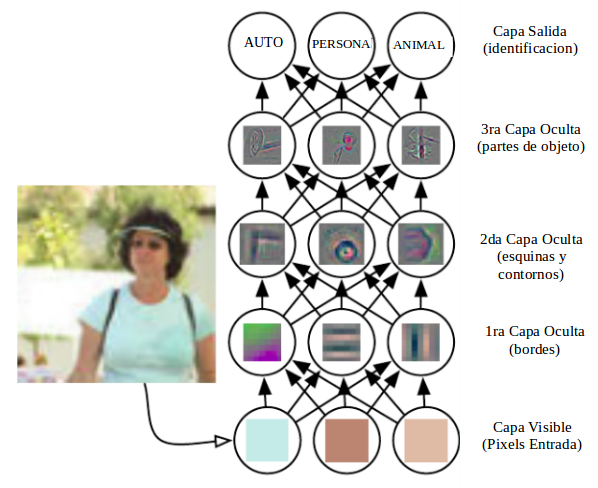
\includegraphics[width=0.7\textwidth]{images/marcoteorico/deepExam}
		\end{center}
		\begin{center}
		\caption{\small{Ilustración de un modelo de aprendizaje profundo}}
		{\small{Fuente propia}}
		\end{center}
		\vspace{-1.5em}
		\end{figure}
	\vskip 0.4cm 
	La idea de aprender la representación correcta de los datos proporciona una perspectiva para el aprendizaje profundo.\citep{Goodfellow-et-al-2016}. Otra perspectiva del aprendizaje profundo es que la profundidad permite que la computadora aprenda un programa de computadora de varios pasos. Cada capa de la representación se puede considerar como el estado de la memoria del computador después de ejecutar otro conjunto de instrucciones en paralelo. Las redes con mayor profundidad pueden ejecutar más instrucciones en secuencia. Las instrucciones secuenciales ofrecen gran poder porque las instrucciones posteriores pueden referirse a los resultados de instrucciones anteriores. De acuerdo con esta visión del aprendizaje profundo, no toda la información en las activaciones de una capa necesariamente codifica los factores de variación que explican la entrada. La representación también almacena información del estado que ayuda a ejecutar un programa el cual puede dar sentido a la entrada. Esta información de estado podría ser análoga a un contador o puntero en un programa informático tradicional. No tiene nada que ver con el contenido de la entrada específicamente, pero ayuda al modelo a organizar su procesamiento.
	\vskip 0.4cm 
	Hay dos formas principales de medir la profundidad de un modelo, \citep{Goodfellow-et-al-2016}. La primera vista se basa en la cantidad de instrucciones secuenciales que se deben ejecutar para evaluar la arquitectura. Podemos considerar esto como la longitud de la ruta más larga a través de un diagrama de flujo que describe cómo calcular cada una de las salidas del modelo a partir de sus entradas. Otro enfoque, utilizado por modelos probabilísticos profundos, considera que la profundidad de un modelo no es la profundidad del gráfico computacional sino la profundidad del gráfico que describe cómo los conceptos se relacionan entre sí. En este caso, la profundidad del diagrama de flujo de los cálculos necesarios para calcular la representación de cada concepto puede ser mucho más profunda que la gráfica de los conceptos mismos. Esto se debe a que la comprensión del sistema de los conceptos más simples puede ser refinado dada la información sobre conceptos más complejos.
	\vskip 0.4cm 
	Debido a que no siempre está claro cuál de estos dos puntos de vista (la profundidad del gráfico computacional o la profundidad del gráfico de modelado probabilístico) es más relevante, y debido a que diferentes personas eligen diferentes conjuntos de elementos más pequeños para construir sus gráficos, no hay un solo valor correcto para la profundidad de una arquitectura, así como no hay un solo valor correcto para la longitud de un programa de computadora. Tampoco hay consenso sobre la profundidad que requiere un modelo para calificar como "profundo", \citep{Goodfellow-et-al-2016}. Sin embargo, el aprendizaje profundo puede considerarse con seguridad como el estudio de modelos que implican una mayor cantidad de composición de funciones o conceptos aprendidos en comparación con el aprendizaje automático tradicional.
	\vskip 0.4cm 
	En resumen, el aprendizaje profundo, es un enfoque a la IA. Específicamente, es un tipo de aprendizaje automático, una técnica que permite que los sistemas computacionales mejoren con la experiencia y los datos. Se puede sostener que el aprendizaje automático es el único enfoque viable para construir sistemas de inteligencia artificial que puedan operar en entornos complicados del mundo real. El aprendizaje profundo es un tipo particular de aprendizaje automático que logra gran poder y flexibilidad al representar el mundo como una jerarquía de conceptos anidados, con cada concepto definido en relación con conceptos más simples y representaciones más abstractas calculadas en base a representaciones menos abstractas. La siguiente es un diagrama de Venn que muestra cómo el aprendizaje profundo es una especie de aprendizaje de representación, que a su vez es una especie de aprendizaje automático, que se utiliza para muchos, pero no todos los enfoques de la IA. 

	\begin{figure}[H]
		\begin{center}
		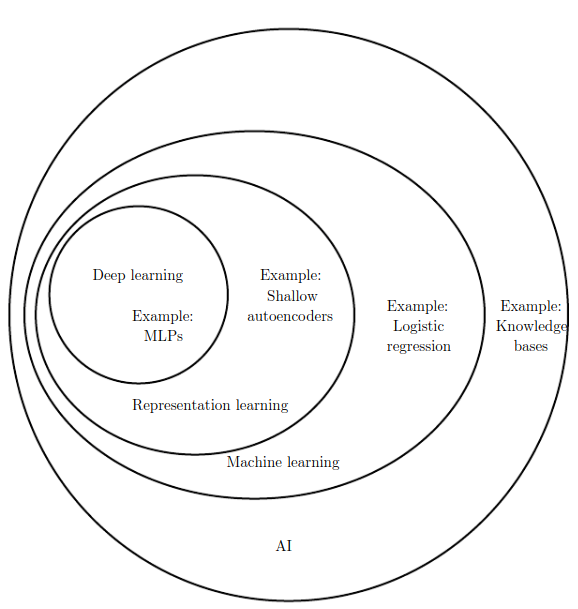
\includegraphics[width=0.8\textwidth]{images/marcoteorico/venn_diag}
		\end{center}
		\begin{center}
		\caption{\small{Diagrama de Venn donde cada sección incluye un ejemplo de una tecnología de IA(ilustra la relación entre estas diferentes disciplinas de la IA)}}
		{\small{Fuente: \citep{Goodfellow-et-al-2016}}}
		\end{center}
		\vspace{-1.5em}
		\end{figure}

\section{Red Convolucional} 

	Nueve de cada diez veces, cuando se escucha que el aprendizaje profundo rompe una nueva barrera tecnológica, las redes neuronales convolucionales están involucradas. También llamados CNN(del inglés , {\bf Convolutional Neural Networks}) o  {\bf ConvNets}, estas son las preferidas del campo de redes neuronales profundas. Han aprendido a clasificar las imágenes en categorías incluso mejor que los humanos en algunos casos, \citep{Rohrer}.
	\vskip 0.4cm  
	Las arquitecturas de redes convolucionales siempre suponen explícitamente que las entradas deben ser mapeadas en forma de imágenes, lo que nos permite configurar parte inicla de las propiedades o características de la arquitectura a diseñar.  Debido a esta característica la limitación de las ConvNets radica en que solo capturan patrones espaciales locales en datos. Es decir, si no se puede hacer que los datos se vean como una imagen, las ConvNets son practicamente muy poco útiles,\citep{Rohrer}.

	\vskip 0.4cm  
	Las redes neuronales convolucionales son muy similares a las redes neuronales ordinarias, están formadas por neuronas que tienen pesos y biases(sesgos) que se pueden aprender. Cada neurona recibe algunas entradas, realiza operaciones matemáticas. Toda la red expresa una única función de puntuación diferenciable: desde el contenido de los píxeles de la imagen en un extremo(entrada) hasta los puntajes que definen la clase o resultado correspondiente en el otro extremo(salida).

	\begin{figure}[H]
	\begin{center}
	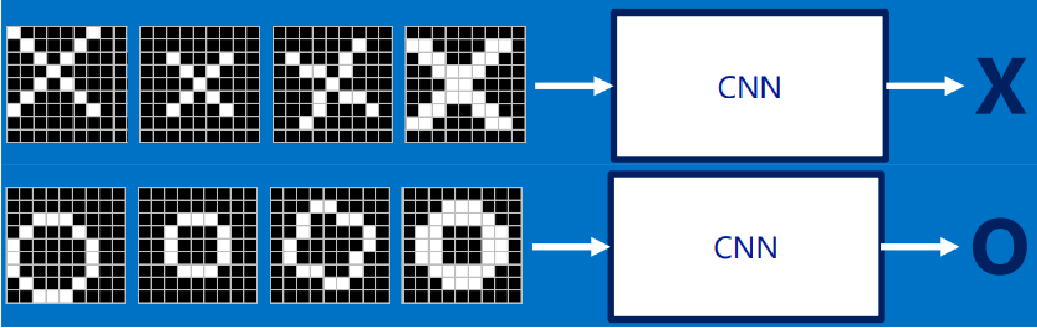
\includegraphics[width=0.7\textwidth]{images/marcoteorico/entr_salida}
	\end{center}
	\begin{center}
	\caption{\small{Entrada y salida de una CNN}}
	{\small{Fuente: \citep{Rohrer}}}
	\end{center}
	\vspace{-1.5em}
	\end{figure}

	El resultado de las CNNs es que pueden encontrar si una característica está en una imagen sin preocuparse exactamente de donde está. Esto ayuda a resolver el problema de las computadoras al comparar imagenes de manera hiper-literal, es decir, que coincida pixel a pixel para que se trate de imágenes iguales.

	\begin{figure}[H]
	\begin{center}
	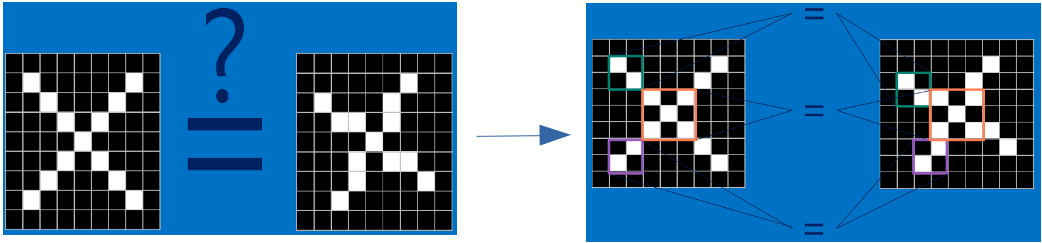
\includegraphics[width=0.8\textwidth]{images/marcoteorico/literalcomp}
	\end{center}
	\begin{center}
	\caption{\small{Analisis de una CNN}}
	{\small{Fuente: \citep{Rohrer}}}
	\end{center}
	\vspace{-1.5em}
	\end{figure}

	Una ConvNet se caracteriza por tener una secuencia de capas donde cada una de estas transforma un volumen de activaciones en otro nuevo a través de una función diferenciable, el aprendizaje profundo se produce cuando se utilizan varias de estas capas variando los parámetros de configuación dentro y entre dichas capas. 
	\vskip 0.4cm  
	Existen dos conjuntos de terminologías para describir estas capas. Una es cuando la red convolucional es vista como 
	un número largo de capas simples y cada paso del procesamiento se considera como una capa en sí misma. Otra terminología es cuando la red convolucional es vista como un número pequeño de capas relativamente complejas, donde cada capa tiene multiples etapas. En esta terminología, existe un mapeo directo entre los volumenes de activaciones y las capas de red. En esta investigación se usará esta terminología.

	
	\begin{figure}[H]
	\begin{center}
	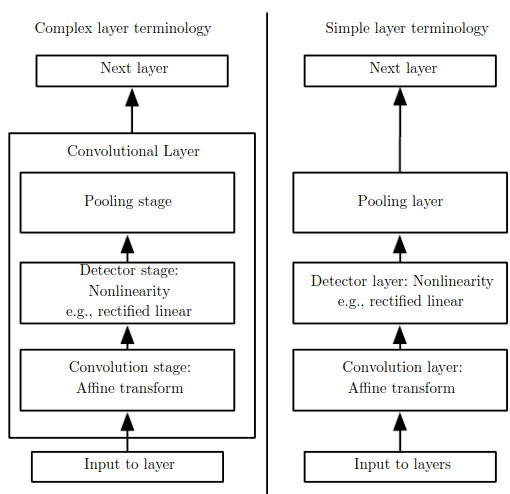
\includegraphics[width=0.6\textwidth]{images/marcoteorico/types}
	\end{center}
	\begin{center}
	\caption{\small{Terminología de capas complejas(izquierda) y de capas simples(derecha)}}
	{\small{Fuente: \citep{Goodfellow-et-al-2016}}}
	\end{center}
	\vspace{-1.5em}
	\end{figure}
	
	\subsection{Capa Convolucional}

		Los parámetros de la capa convolucional consisten basicamente en dos datos. La entrada y todo lo que respecta a un conjunto de filtros(también denomidados kernels) cuyos valores se aprenden, es decir, empiezan con datos aleatorios y conforme avance el entrenamiento se van alterando. 
		\vskip 0.3cm 
		\subsubsection {Etapa de Convolución} 
		  
		Para el proceso convolucional cada filtro es pequeño espacialmente (a lo ancho y alto), incluso se extiende a través de la profundidad total del volumen de entrada(imagen). Por ejemplo, un filtro típico en una primera capa de una ConvNet podría tener un tamaño de 5x5x3 (es decir, 5 píxeles de ancho y alto, y 3 de profundidad debido a que los canales de color - RGB). Durante el proceso hacia adelante, se desliza (más precisamente, convolve) cada filtro a través del ancho y alto(incluso produnfidad) del volumen de entrada para calcular los productos de puntos entre las entradas del filtro y la entrada en cualquier posición.

		\begin{figure}[H]
		\begin{center}
		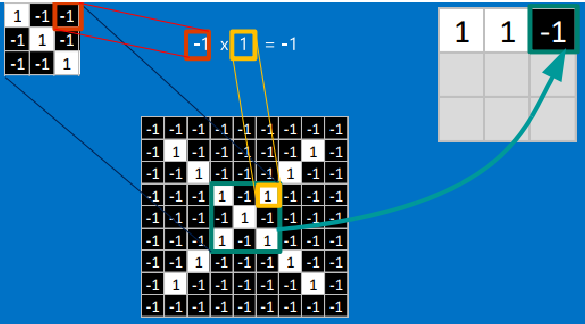
\includegraphics[width=0.75\textwidth]{images/marcoteorico/generate_filt1}
		\end{center}
		\begin{center}
		\caption{\small{Convolucion entre el filtro y parte de la imagen}}
		{\small{Fuente: \citep{Rohrer}}}
		\end{center}
		\vspace{-1.9em}
		\end{figure}

		\begin{figure}[H]
		\begin{center}
		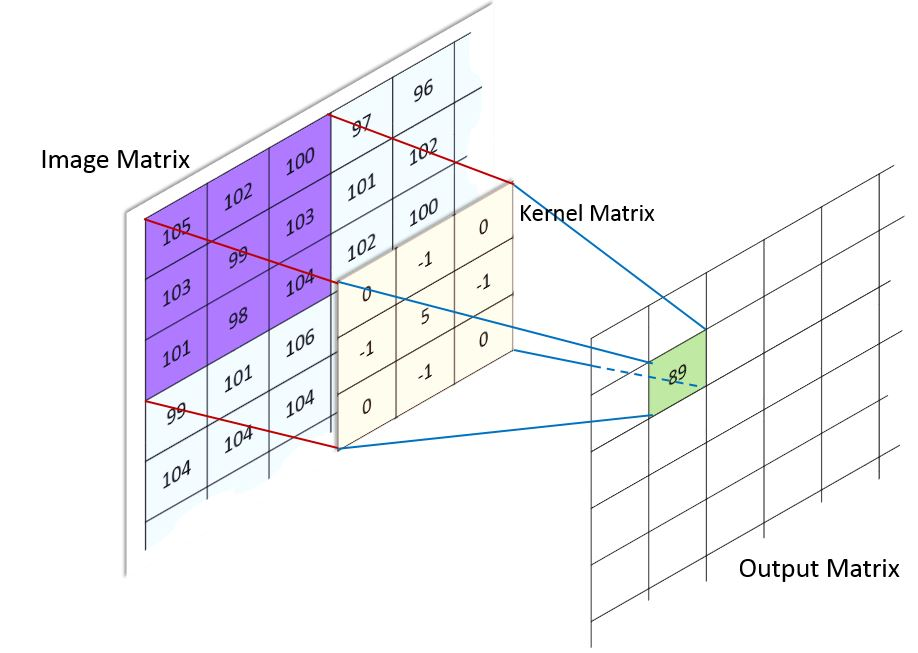
\includegraphics[width=0.75\textwidth]{images/marcoteorico/Convolution_calculation1}
		\end{center}
		\begin{center}
		\caption{\small{Posicionamiento del kernel/filtro por pixel}}
		{\small{Fuente: Fuente Propia}}
		\end{center}
		\vspace{-1.9em}
		\end{figure}

		A medida que deslizamos el filtro sobre el ancho y la altura del volumen de entrada produciremos un mapa de activación bidimensional que proporciona las respuestas de ese filtro en cada posición espacial. Es decir, el proceso en esta capa consiste en calcular la coincidencia de un filtro con una parte de la imagen,y para conseguirlo simplemente se multiplica cada píxel en el filtro por el valor del píxel en la imagen. Para luego, sumar las respuestas y dividirlas por el número total de píxeles en el filtro.

		\begin{figure}[H]
		\begin{center}
		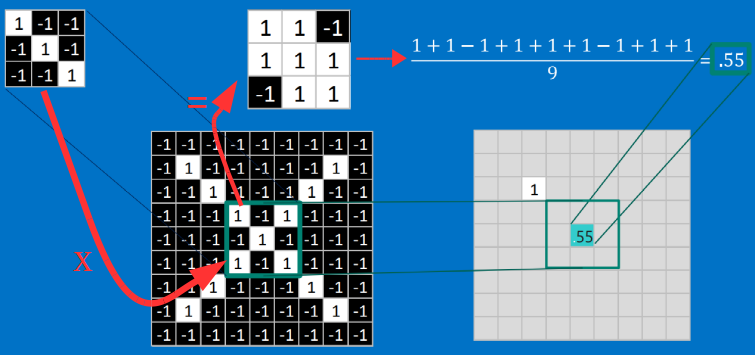
\includegraphics[width=0.75\textwidth]{images/marcoteorico/conv_filt1}
		\end{center}
		\begin{center}
		\caption{\small{Proceso matemático convolucional}}
		{\small{Fuente:\citep{Rohrer}}}
		\end{center}
		\vspace{-1.5em}
		\end{figure}

		\begin{figure}[H]
		\begin{center}
		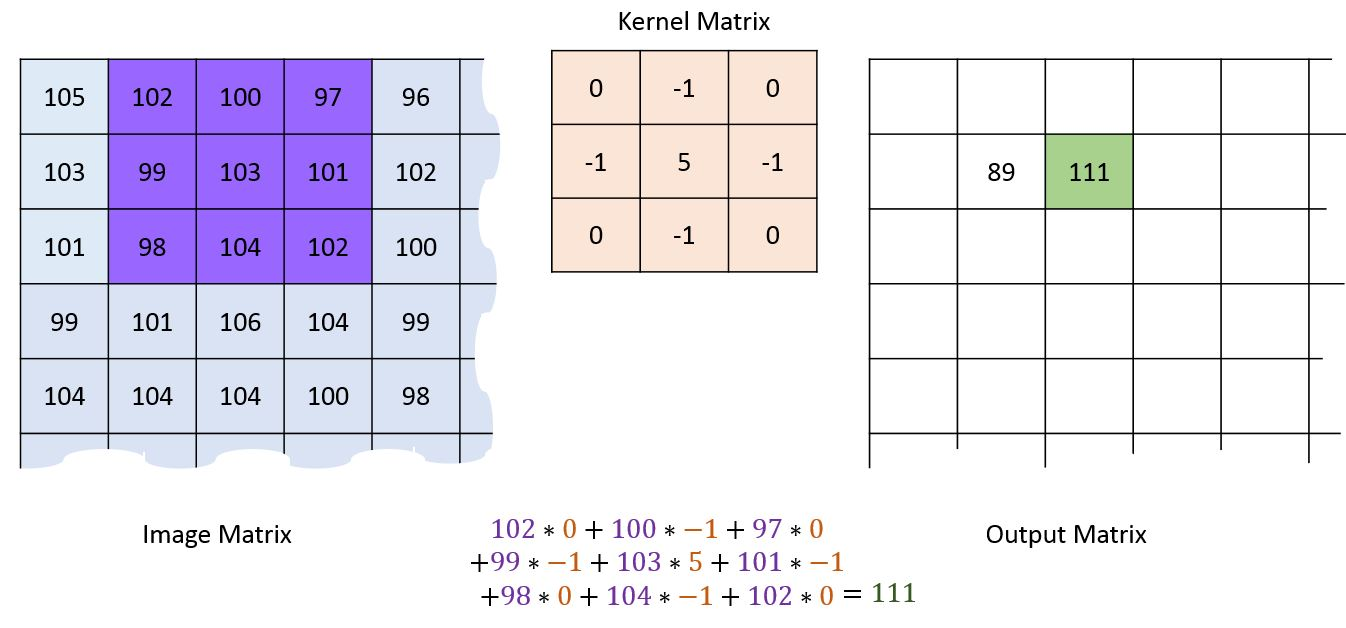
\includegraphics[width=0.75\textwidth]{images/marcoteorico/Convolution_calculation2}
		\end{center}
		\begin{center}
		\caption{\small{Cálculo Convolucional}}
		{\small{Fuente: Fuente Propia}}
		\end{center}
		\vspace{-1.9em}
		\end{figure}

		Cada filtro puede ser representado como una neurona de salida, cuyo valor se halla usando la sumatoria de pesos como se muestra en la figura 11. Intuitivamente, la red aprenderá los filtros que se activan cuando ven algún tipo de característica visual, como un borde o contorno en alguna orientación específica. 
		
		\vskip 0.4cm  
		
		La convolución aprovecha tres ideas importantes que pueden ayudar a mejorar un sistema de aprendizaje automático: {\bf interacciones dispersas, uso compartido de parámetros} y {\bf representaciones equivalentes}.
		
		\vskip 0.4cm  
		Las capas de redes neuronales tradicionales usan la multiplicación de matrices mediante una matriz de parámetros con un parámetro separado que describe la interacción entre cada unidad de entrada y cada unidad de salida. Esto significa que cada unidad de salida interactúa con cada unidad de entrada. Sin embargo, las redes convolucionales suelen tener {\bf interacciones dispersas} (también conocidas como conectividad dispersa o ponderaciones dispersas). Esto se logra haciendo que el kernel sea más pequeño que la entrada. Por ejemplo, al procesar una imagen, la imagen de entrada puede tener miles o millones de píxeles, pero podemos detectar características pequeñas y significativas, como bordes con núcleos que ocupan solo decenas o cientos de píxeles. Esto significa que necesitamos almacenar menos parámetros, lo que reduce los requisitos de memoria del modelo y mejora su eficiencia estadística. También significa que el cálculo de la salida requiere menos operaciones.
		
		\begin{figure}[H]
		\begin{center}
		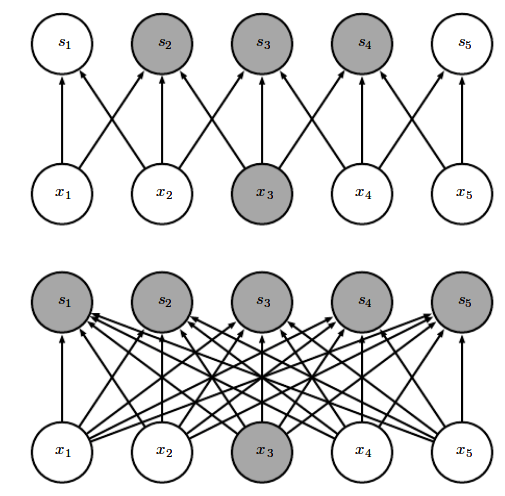
\includegraphics[width=0.5\textwidth]{images/marcoteorico/sparceCon}
		\end{center}
		\begin{center}
		\caption{\footnotesize \small{Conectividad dispersa}}
		{\small{Fuente:\citep{Rohrer}}}
		\end{center}
		\vspace{-1.5em}
		\end{figure} 	

		Estas mejoras en la eficiencia suelen ser bastante grandes. Si hay entradas y salidas, la multiplicación de la matriz requiere $m \times n$ parámetros, y los algoritmos utilizados en la práctica por ejemplo tienen complejidad de tiempo de ejecución $O(m \times n)$. Si limitamos el número de conexiones que cada salida puede tener a {\textit k}, entonces el enfoque dispersamente conectado requiere solo $k \times n$ parámetros y $O(k \times n)$ en tiempo de ejecución. Para muchas aplicaciones prácticas, es posible obtener un buen rendimiento en la tarea de aprendizaje automático mientras se mantienen {\textit k} distintos órdenes de magnitud menores que {\textit m}. Para demostraciones gráficas de conectividad dispersa, vea la figura X, donde se resalta una unidad de entrada $x_{3}$, y las unidades de salida que son afectadas por esta unidad. (Arriba) Cuando {\textit \bf s} está formado por convolución con un kernel de ancho 3, solo tres salidas se ven afectadas por {\textit \bf x}. (Abajo) Cuando {\textit \bf s} está formado por la multiplicación de la matriz, la conectividad ya no es dispersa, por lo que todos los resultados se ven afectados por $x_{3}$.

		\vskip 0.4cm  
		En una red convolucional profunda, las unidades en las capas más profundas pueden interactuar indirectamente con una porción más grande de la entrada. Esto permite que la red describa de manera eficiente las interacciones complicadas entre muchas variables mediante la construcción de tales interacciones a partir de bloques de construcción simples que describen cada una de ellas. Entonces, aunque las conexiones directas en una red convolucional son muy dispersas, las unidades en las capas más profundas pueden conectarse indirectamente a la totalidad o a la mayoría de la imagen de entrada.
		
		\vskip 0.4cm  
		
		El uso {\bf compartido de parámetros} hace referencia al uso del mismo parámetro para más de una función en un modelo. En una red neuronal tradicional, cada elemento de la matriz de pesos se usa exactamente una vez cuando se calcula la salida de una capa. Se multiplica por un elemento de la entrada y luego nunca se vuelve a visitar. Como sinónimo de compartir parámetros, se puede decir que una red hastió pesas, porque el valor del peso aplicado a una entrada está vinculado al valor de una ponderación aplicada en donde. En una red neuronal convolucional, cada miembro del kernel se utiliza en cada posición de la entrada (excepto tal vez algunos de los píxeles del límite, dependiendo de las decisiones de diseño con respecto al límite). El uso compartido de parámetros utilizado por la operación de convolución significa que en lugar de aprender un conjunto separado de parámetros para cada ubicación, aprendemos solo un conjunto.
		\vskip 0.4cm  

		En el caso de la convolución, la forma particular de compartir los parámetros hace que la capa tenga una propiedad llamada {\bf representaciones equivalentes}. Decir que una función es equivalente significa que si la entrada cambia, la salida cambia de la misma manera.
		La convolución crea un mapa en 2-D de donde aparecen ciertas características en la entrada. Si movemos el objeto en la entrada, su representación se moverá la misma cantidad en la salida. Esto es útil cuando sabemos que se utiliza alguna función de un número pequeño de píxeles vecinos cuando se aplica a ubicaciones de entrada múltiples. Por ejemplo, al procesar imágenes, es útil detectar bordes en la primera capa de una red convolucional. Los mismos bordes aparecen más o menos en todas partes en la imagen, por lo que es práctico compartir los parámetros en toda la imagen.

		\begin{figure}[H]
		\begin{center}
		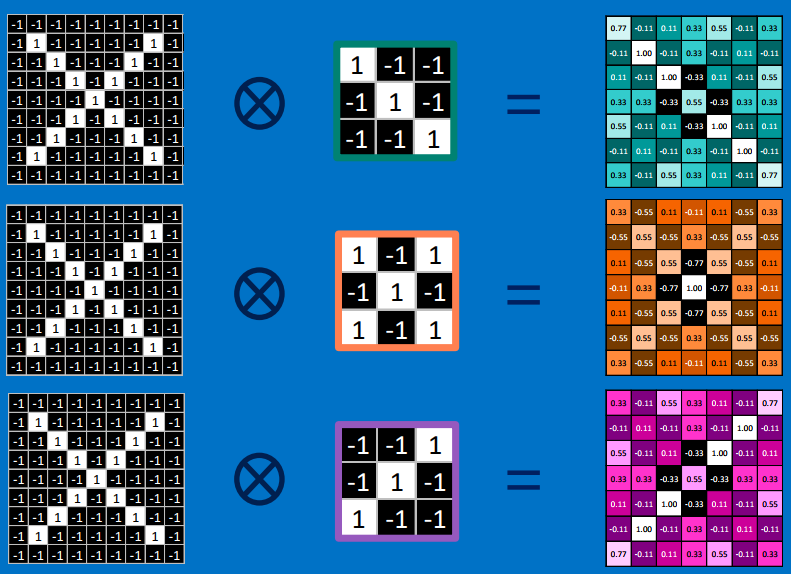
\includegraphics[width=0.6\textwidth]{images/marcoteorico/result_conv}
		\end{center}
		\begin{center}
		\caption{\small{Resultado de Convolución(conjunto de mapas de activación. generado a partir de 3 filtros para 3 carecteristicas: diagonal derecha, cruzamiento central y diagonal izquierda). Simbolo de convolución: $\otimes$}}
		{\small{Fuente: \citep{Rohrer}}}
		\end{center}
		\vspace{-1.9em}
		\end{figure}

		En resumen, se tiene un conjunto completo de "n" filtros en cada capa convolucional(determinando la profundidad de la capa) y cada uno de estos filtros producirá un mapa de activación bidimensional por separado. Apilaremos estos mapas de activación a lo largo de la dimensión de profundidad y produciremos el volumen de salida, es decir el resultado es un conjunto de imágenes que muestran un versión filtrada de la imagen original resaltando características o patrones importantes de ella, como puede ser visto en la figura 14.

		\vskip 0.4cm  
		Cabe resaltar que para la construcción de un filtro o kernel, es necesario considerar tres aspectos importantes: la extensión espacial (spatial extent), el paso (stride) y la cantidad de zero a rellenar (zero-padding).
		\vskip 0.4cm  
		
		\begin{enumerate}
			\item La extensión espacial es el tamaño del filtro, comúnmente es de tamaño impar tanto en largo y ancho.
			
			\item El stride es otra pieza del bloque de construcción básico de los filtros convolucionales. Este representa el {\textit 'paso'} en la operación de convolución indicando cuánto es que se debe desplazar un filtro en una imagen con cada paso. El filtro se desliza sobre la imagen, se detiene en cada longitud de salto y realiza las operaciones necesarias en ese paso.

			\begin{figure}[H]
			\begin{center}
			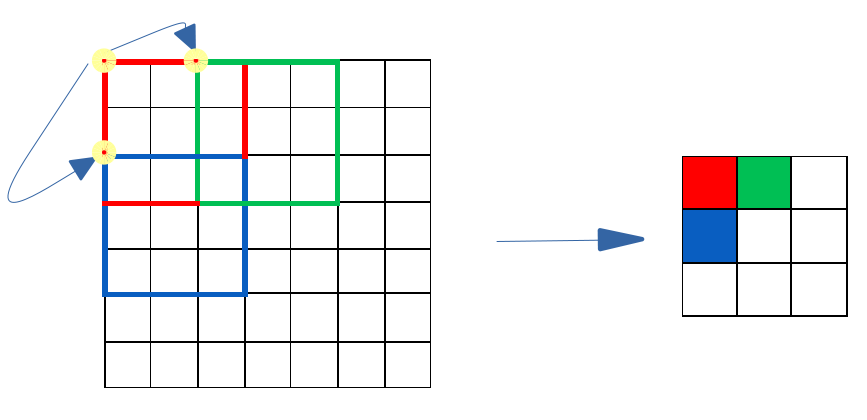
\includegraphics[width=0.65\textwidth]{images/marcoteorico/stride}
			\end{center}
			\begin{center}
			\caption{\small{Imagen con stride igual a 2, para el filtro tanto en largura como anchura}}
			{\small{Fuente propia}}
			\end{center}
			\vspace{-1.9em}
			\end{figure}

			\item Zero-padding agrega ceros alrededor del borde de una imagen.
			\begin{figure}[H]
			\begin{center}
			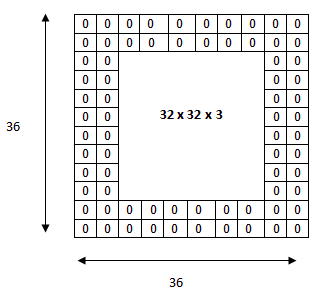
\includegraphics[width=0.4\textwidth]{images/marcoteorico/PAD2}
			\end{center}
			\begin{center}
			\caption{\small{Ejemplo de zero-padding con tamaño 2}}
			{\small{Fuente propia}}
			\end{center}
			\vspace{-1.9em}
			\end{figure}

			Los principales beneficios del relleno son los siguientes:
			\begin{itemize}
			\item Le permite usar una capa de convolución sin necesariamente reducir la altura y el ancho de los volúmenes. Esto es importante para construir redes más profundas, ya que de lo contrario la altura / ancho se reduciría a medida que se avanza hacia capas más profundas.
			\item Nos ayuda a mantener más información en el borde de una imagen. Sin relleno, muy pocos valores en la siguiente capa se verían afectados por los píxeles como los bordes de una imagen.
			\end{itemize}
			
		\end{enumerate}
		%\vskip 0.4cm  

		\noindent Cada capa convolucional recibe como dato de entrada llos parámetros:
		${W_{0}}\times{H_{0}}\times{D_{0}}$ \newline
		Produce un dato de salida con los siguiente parámetros: ${W_{1}}\times{H_{1}}\times{D_{1}}$\newline
		Estas salidas, son influenciadas por la manera de configuración de los filtros.\newline
		\vskip 0.1cm 
		
		\begin{minipage}[t]{0.5\textwidth}
		En el que:
		\begingroup\makeatletter\def\f@size{12.4}\check@mathfonts
		\begin{center}
		 ${W_{1}} = \frac{{W_{0}} - F + 2P}{S} +1$ 
		\vskip 0.4cm 
		 ${H_{1}} = \frac{{H_{0}} - F + 2P}{S} +1$ 
		\vskip 0.4cm 
		 ${D_{1}} = K$ 
		 \end{center}
		\endgroup
		\end{minipage}
		%second column
		\begin{minipage}[t]{0.55\textwidth}
		Donde:
		\vskip 0.1cm 
		$W$ es el ancho (width) de la imagen, \vskip 0.4cm  
		$H$ es la altura (height) de la imagen,\vskip 0.4cm 
		$D$ es la profundidad (depth)de la imagen,\vskip 0.4cm 
		$F$ es la extensión espacial (spatial extent) del filtro,\vskip 0.4cm 
		$S$ es el paso (stride) del filtro,\vskip 0.4cm 
		$P$ es la cantidad de zero padding del filtro,\vskip 0.4cm 
		$K$ es el número de filtros (filters).\vskip 0.4cm 
		\end{minipage}
		\vskip 0.4cm 
		\noindent La ecuación de convolución de manera generalizada es:
		
		\begingroup\makeatletter\def\f@size{14.4}\check@mathfonts
		\begin{center}
		${conv_j^n} ={\sum_{k=1}^k x_k^n \times w_{kj} ^n + b_n}$
		\end{center}
		\endgroup
		
		En el que:\vskip 0.1cm
		\begin{itemize}
			\item $x,w,b$ son valores de entrada, pesos y biases(sesgos), respectivamente
			\item $n$ es el número de la capa
			\item $j$ es el número del filtro de salida
			\item $k$ es la cantidad de filtros en la capa $n-1$ o $n$
		\end{itemize}


		\begin{figure}[H]
		\begin{center}
		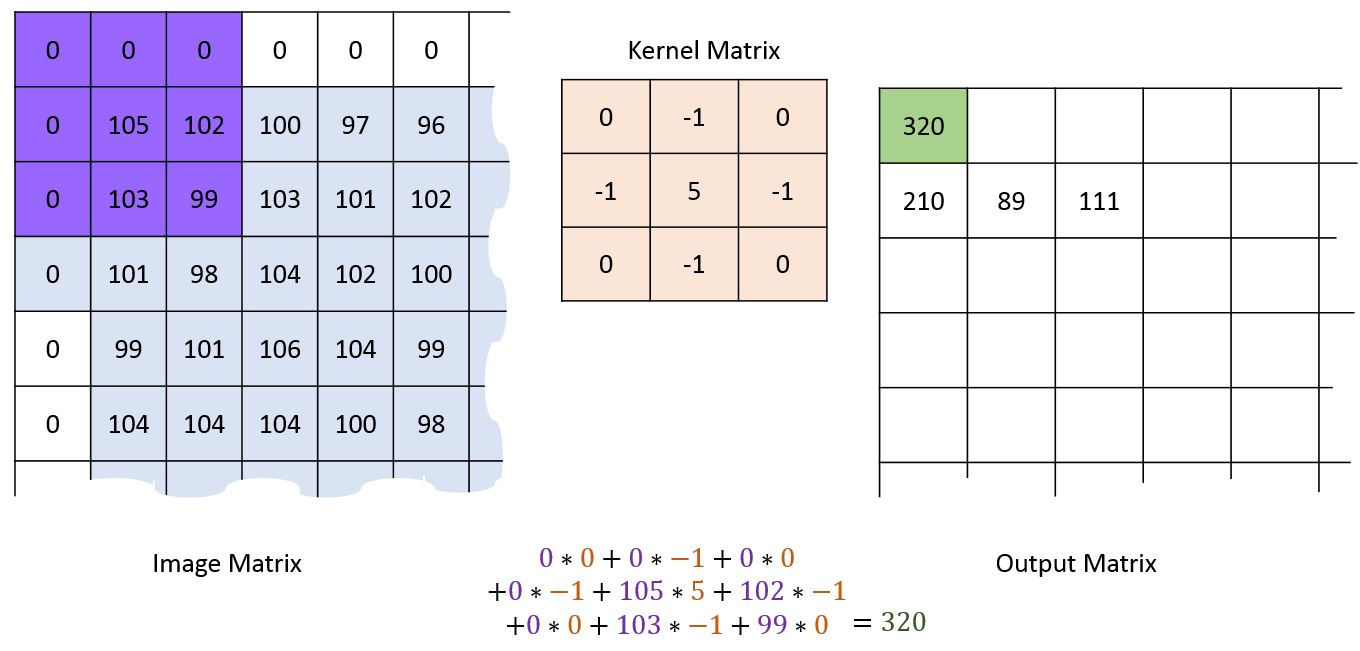
\includegraphics[width=0.9\textwidth]{images/marcoteorico/Convolution_calculation_borders}
		\end{center}
		\begin{center}
		\caption{\small{Ejemplo de filtro crado apartir de los 3 aspectos mencionados}}
		{\small{Fuente propia}}
		\end{center}
		\vspace{-1.9em}
		\end{figure}

	%\vskip 0.4cm 
	\subsubsection  {Capa ReLU(Rectified Linear Units)}
		\vskip 0.4cm 
		Debido al hecho que todas las capas en una red neuronal no son lineales. Después de calcular los valores para cada una de las neuronas en la red neuronal, colocamos estos valores a través de una función de activación. Una red neuronal artificial consiste básicamente en multiplicaciones y suma de matrices. Si solo utilizáramos estos cálculos lineales, podríamos apilarlos uno encima del otro y esa no sería una red muy profunda. Por lo tanto, a menudo se utiliza funciones de activación no lineales en cada capa de la red. Al apilar capas de funciones lineales y no lineales una encima de la otra, teóricamente podemos modelar cualquier problema.
		\vskip 0.4cm 
		Estas son las tres funciones de activación no lineal más populares:
		\begin{enumerate}
		\item[1)] Sigmoid (analiza un valor entre 0 y 1)  \vspace{-0.5em}
		\item[2)] TanH (analiza un valor entre -1 y 1) \vspace{-0.5em}
		\item[3)] ReLU (si el valor es negativo, se convierte en 0, de lo contrario, permanece igual) \vspace{-0.5em}
		\end{enumerate}

		\begin{figure}[H]
		\begin{center}
		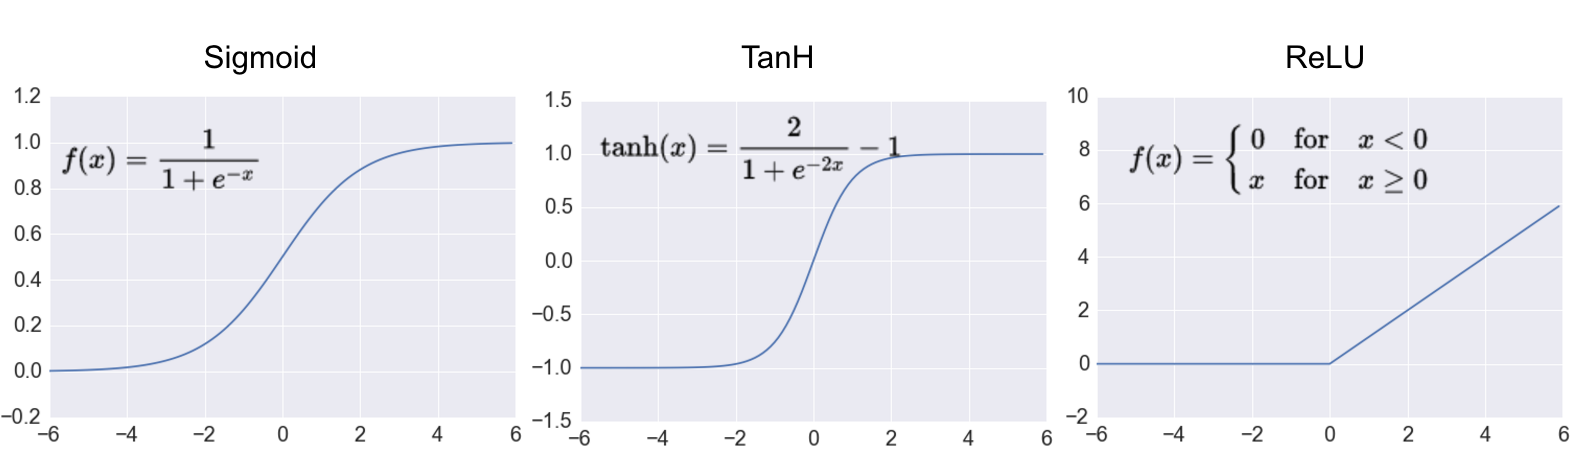
\includegraphics[width=0.8\textwidth]{images/marcoteorico/activfunct}
		\end{center}
		\begin{center}
		\caption{\small{Funciones de activación}}
		{\small{Fuente propia}}
		\end{center}
		\vspace{-1.5em}
		\end{figure}

		Actualmente, ReLU es la función de activación no lineal más utilizada \citep{cs231n}. La razón principal de esto es porque la red puede entrenar mucho más rápido (debido a la eficiencia computacional) sin hacer una diferencia significativa en la precisión. También ayuda a aliviar el problema del gradiente de fuga, que es el problema donde las capas inferiores de la red entrenan muy lentamente porque el gradiente de optimización	disminuye exponencialmente a través de las capas. La capa ReLU aplica la función ${f(x)} = {max (0, x)} $ a todos los valores en el volumen de entrada. En términos básicos, esta capa simplemente cambia todas las activaciones negativas a 0. Esta capa aumenta las propiedades no lineales del modelo y la red global sin afectar los campos receptivos de la capa conv. El hecho de que entradas en la función de activación de valores menores o iguales a cero resulten cero, induce a la dispersión en las unidades ocultas, que según lo comentado anteriormente, produce representaciones dispersas las cuales se consideran más valiosas, \citep{RELU}. 
		
		\begin{figure}[H]
		\begin{center}
		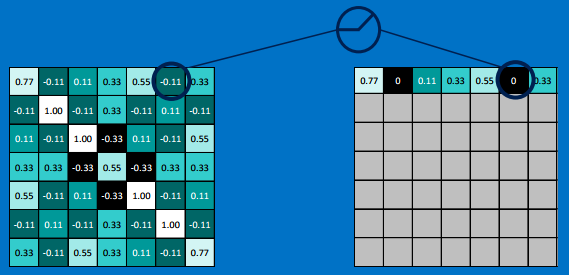
\includegraphics[width=0.8\textwidth]{images/marcoteorico/relu}
		\end{center}
		\begin{center}
		\caption{\small{Procedimiento de la función ReLU}}
		{\small{Fuente: \citep{Rohrer}}}
		\end{center}
		\vspace{-1.5em}
		\end{figure}
		\vskip 0.4cm
		
		Es por ello que entre la capa(etapa) de convolucion y la capa(etapa) de pooling puede encontrarse la capa ReLU que esta compuesta por neuronas que poseen una funcion de activación llamada Función Lineal Rectificada que deriva de la función de activación sigmoidal, pero tiene mayores ventajas que esta última y tambien de la tangencial. Las activaciones de ReLU se sobreponen más fácilmente que los sigmoides, esto los prepara muy bien para ser utilizados en combinación con la técnica DROPOUT.
		
		\vskip 0.4cm 
	\subsubsection {Técnica Dropout}
		\vskip 0.4cm 
		Combinar las predicciones de muchos modelos diferentes es una forma muy exitosa de reducir los errores de prueba, pero parece ser demasiado costoso para las redes neuronales de gran tamaño debido a que pueden tardar varios días en entrenar. Sin embargo, dropout es una técnica de regularización que tiene por objetivo de reducir el sobreajuste que puede darse durante el entrenamiento de una red neuronal. Consiste en establecer a cero la salida de cada neurona oculta con una probabilidad 0.5(comúnmente). Las neuronas que se "abandonan" de esta manera no contribuyen al pase directo y no participan en las siguientes etapas de entrenamiento.

		\begin{figure}[H]
		\begin{center}
		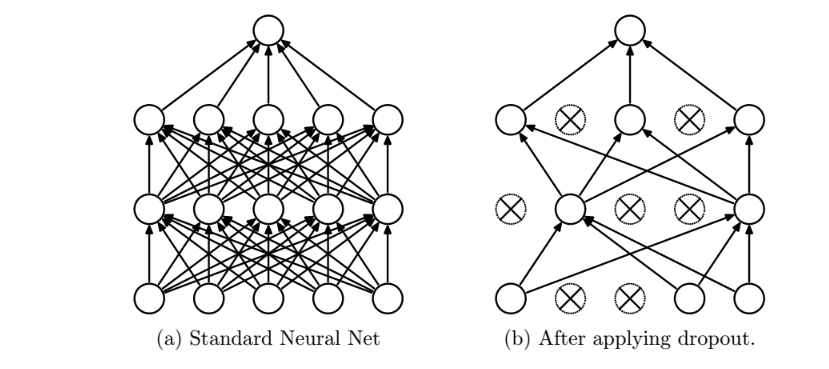
\includegraphics[width=0.8\textwidth]{images/marcoteorico/dropout_sample}
		\end{center}
		\begin{center}
		\caption{\small{En la izquierda la red neuronal común y a la derecha la red neuronal diluida producida por la aplicación de dropout}}
		{\small{\citep{AulaDNN}}}
		\end{center}
		\vspace{-1.5em}
		\end{figure}
		

		\vskip 0.4cm 
		Por lo tanto, cada vez que se presenta una entrada, la red neuronal muestrea una arquitectura diferente, pero todas estas arquitecturas comparten ponderaciones. Esta técnica reduce las coadaptaciones complejas de las neuronas, ya que una neurona no puede depender de la presencia de otras neuronas particulares. Por lo tanto, se ve forzado a aprender características más robustas que son útiles en conjunción con muchos subconjuntos aleatorios diferentes de las otras neuronas.
		\begin{figure}[H]
		\begin{center}
		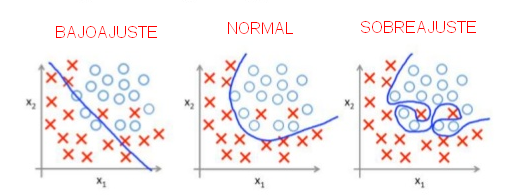
\includegraphics[width=0.8\textwidth]{images/marcoteorico/dropout}
		\end{center}
		\begin{center}
		\caption{\small{Procesos que pueden ocurrir durante entrenamiento. Dropout evita el sobreajuste}}
		{\small{Fuente propia}}
		\end{center}
		\vspace{-1.5em}
		\end{figure}

		\vskip 0.4cm 
	\subsubsection {Capa de Agrupación(Pooling)}
		\vskip 0.4cm 

		Una variedad de cálculos que reducen la dimensionalidad de un mapa de características se conocen como agrupación. La agrupación, que se aplica a cada canal por separado, permite que la red sea robusta e invariante a pequeños cambios y distorsiones. La capa Pooling(también conocida como una capa de reducción de resolución) combina o agrupa, un conjunto de valores en su campo receptivo en un menor número de valores. Puede ser configurado en función del tamaño de su campo receptivo (por ejemplo, 2 x 2) y en función a la operación de agrupamiento (por ejemplo, máximo-max o promedio-average), como se muestra en Fig. 20. Normalmente, la agrupación se produce en bloques que no se solapan (es decir, el paso o stride es igual al tamaño de la agrupación). Usualmente se usa una stride mayor que uno cuando se quiere que haya una reducción en la dimensión de la representación(mapa de características).

		\begin{figure}[H]
		\begin{center}
		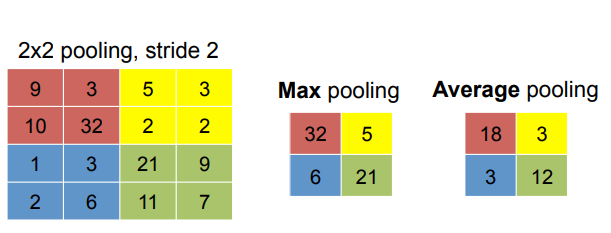
\includegraphics[width=0.8\textwidth]{images/marcoteorico/pooling}
		\end{center}
		\begin{center}
		\caption{\small{Formas de agrupamiento(pooling)}}
		{\small{Fuente: \citep{caffe}}}
		\end{center}
		\vspace{-1.5em}
		\end{figure}

		Después de algunas capas ReLU, es común optar por aplicar una capa de agrupamiento. En esta categoría, la operación MAX(conocida como Max-pooling) es la más popular reduciendo progresivamente el tamaño espacial de la representación de una imágen(mapa de características) mientras conserva la información más importante en ella, esto se ejecuta con dos objetivos, el primero de reducir la cantidad de parámetros y el cálculo en la red. El segundo es que controlará el sobreajuste.
		\vskip 0.4cm 
		La capa de agrupación opera independientemente en cada segmento de profundidad de la entrada y la cambia de tamaño espacialmente(reduce su resolución). El proceso matematico consiste en pasar una pequeña ventana(kernel) através de una imagen y tomar el valor máximo de la ventana en cada paso. 


		\begin{figure}[H]
		\begin{center}
		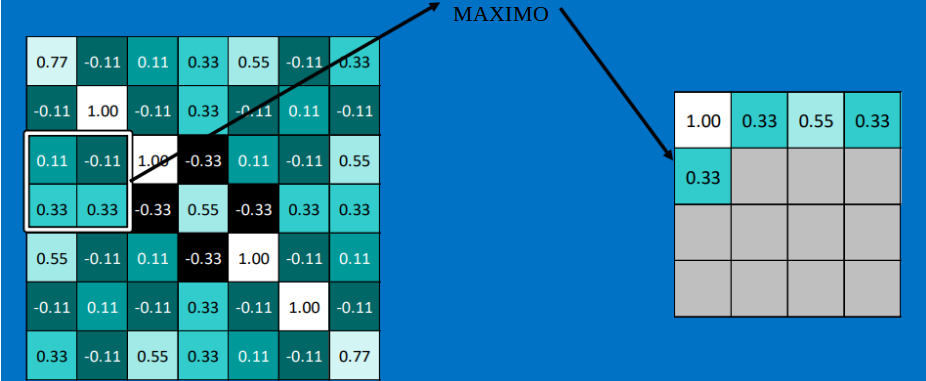
\includegraphics[width=0.75\textwidth]{images/marcoteorico/pool1}
		\end{center}
		\begin{center}
		\caption{\small{Operación MAX-pooling en capa de Agrupación}}
		{\small{Fuente: \citep{Rohrer}}}
		\end{center}
		\vspace{-1.5em}
		\end{figure}

		Este proceso es aplicado para cada mapa de activación(salida de la capa de convolución). Análogamente con la capa de convolución, el resultado en esta capa es un conjunto de imágenes que muestran un versión agrupada de las imágenes de entrada.

		\begin{figure}[H]
		\begin{center}
		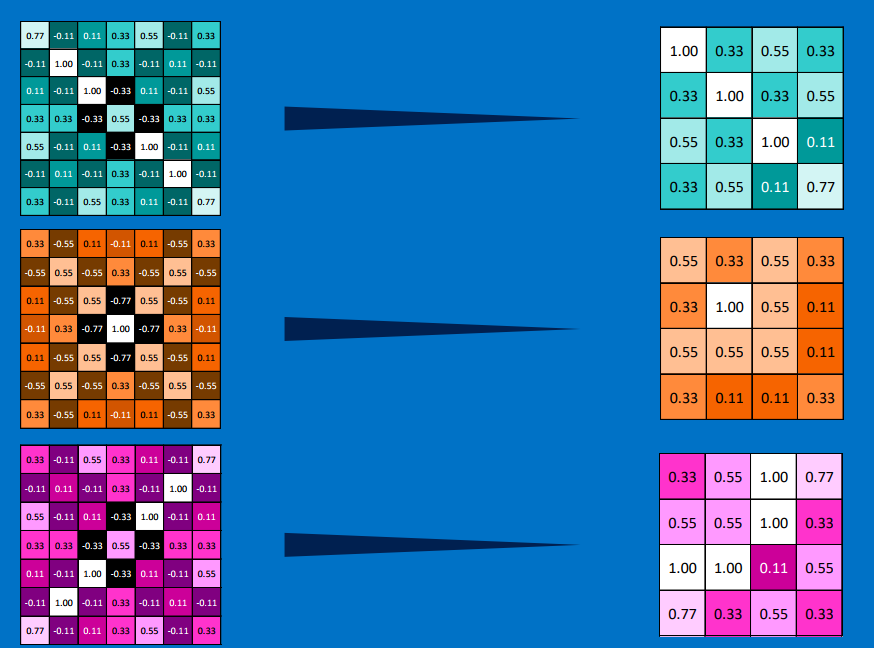
\includegraphics[width=0.7\textwidth]{images/marcoteorico/pool2}
		\end{center}
		\begin{center}
		\caption{\small{Resultado de Agrupación}}
		{\small{Fuente: \citep{Rohrer}}}
		\end{center}
		\vspace{-1.5em}
		\end{figure}


		\noindent Esta capa pooling recibe como dato de entrada los parámetros:
		${W_{0}}\times{H_{0}}\times{D_{0}}$ \newline
		Y produce un dato de salida con los siguiente parámetros: ${W_{1}}\times{H_{1}}\times{D_{1}}$\newline
		
		% first column
		\begin{minipage}[t]{0.5\textwidth}
		En el que:
		\begin{center}
		 ${W_{1}} = \frac{{W_{0}} - F }{S} +1$ 
		\vskip 0.4cm 
		 ${H_{1}} = \frac{{H_{0}} - F }{S} +1$ 
		\vskip 0.4cm 
		 ${D_{1}} = {D_{0}}$ 
		 \end{center}
		\vskip 0.6cm 
		\end{minipage}
		%second column
		\begin{minipage}[t]{0.55\textwidth}
		Donde:
		\vskip 0.1cm 
		$W$ es el ancho (width) de la imagen, \vskip 0.4cm  
		$H$ es la altura (height) de la imagen,\vskip 0.4cm 
		$D$ es la profundidad (depth) de la imagen,\vskip 0.4cm 
		$F$ es la extensión espacial (spatial extent) del kernel,\vskip 0.4cm 
		$S$ es el paso (stride) del kernel,\vskip 0.4cm 
		\end{minipage}

		\begin{figure}[H]
		\begin{center}
		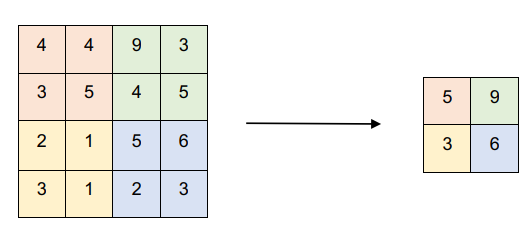
\includegraphics[width=0.5\textwidth]{images/marcoteorico/pool4}
		\end{center}
		\begin{center}
		\caption{\small{Max-pooling con filtro 2x2 y paso 2}}
		{\small{Fuente propia}}
		\end{center}
		\vspace{-1.5em}
		\end{figure}

	\subsection{Capa totalmente conectada (Fully-connected layer)}

		Esta capa por lo general aparece al final de la arquitectura y es similar al Perceptrón multicapa(MultilayerPerceptron -MLP), en el cual la neurona de salida se conecta a todas las neuronas de entrada y el peso de las conexiones son actualizadas usando el método de retropropagación.
		\vskip 0.4cm  
		Eventualmente, con un mapa de características lo suficientemente pequeño, el contenido se aplastará en un vector de una sola dimensión y será entrada para en un MLP totalmente conectado para su procesamiento.
		\vskip 0.4cm  
		Habiendo detallado que la función ReLU es la más utilizada en las capas anteriores, en esta última capa del modelo generalmente se utiliza una función de activación diferente, porque en esta capa se pretende que tenga una salida determinada. La {\bf función softmax} es muy popular cuando se hace la clasificación.
	


	\newpage
	En resumen, una arquitecuta o modelo de red convolucional estará compuesto de varias capas y ejecutará las siguientas actividades:
	\begin{figure}[H]
		\begin{center}
		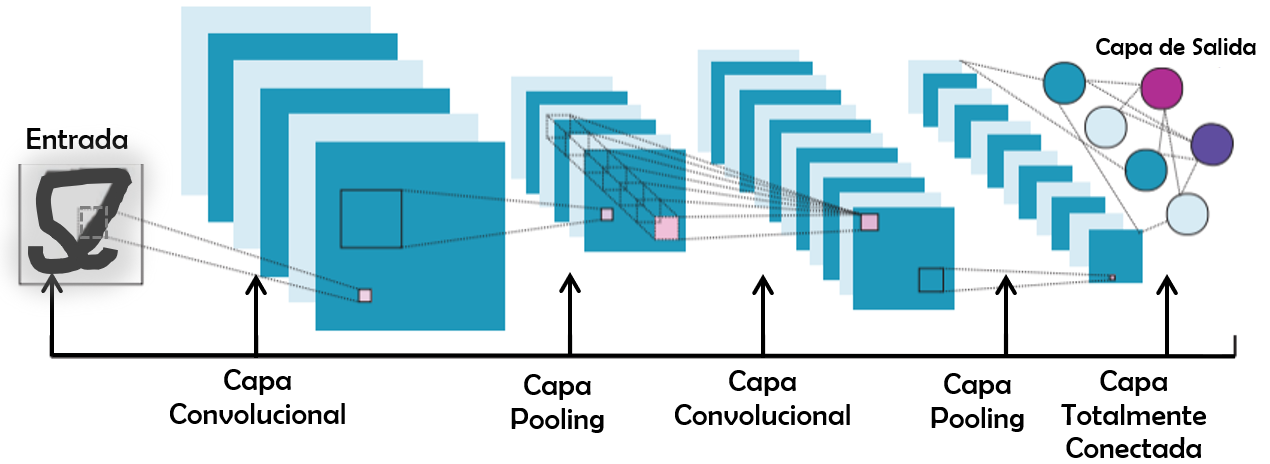
\includegraphics[width=0.8\textwidth]{images/marcoteorico/modelo}
		\end{center}
		\begin{center}
		\caption{\small{Modelo de red neuronal convolucional profunda}}
		{\small{Fuente propia}}
		\end{center}
		\vspace{-1.5em}
		\end{figure}

	\begin{itemize}
		\item Se pasa una imagen de entrada a la primera capa convolucional. La salida complicada se obtiene como un mapa de activación. Los filtros aplicados en la capa de convolución extraen características relevantes de la imagen de entrada para pasar más lejos.\vspace{-0.5em}

		\item Cada filtro dará una característica diferente para ayudar a la predicción de clase correcta. En caso de que necesitemos retener el tamaño de la imagen, usamos el mismo relleno (padding cero), de lo contrario se usa el relleno válido ya que ayuda a reducir el número de características. \vspace{-0.5em}

		\item Las capas de agrupamiento se agregan para reducir aún más el número de parámetros.\vspace{-0.5em}

		\item Se agregan varias capas de convolución y agrupación antes de realizar la predicción. \vspace{-0.5em}

		\item A medida que profundizamos en la red, se extraen características más específicas en comparación con una red superficial donde las características extraídas son más genéricas. \vspace{-0.5em}

		\item La capa de salida en una CNN, como se mencionó anteriormente, es una capa totalmente conectada, donde la entrada de las otras capas se aplana y se envía para transformar la salida en el número de clases que desea la red. \vspace{-0.5em}

		\item La salida se genera a través de la capa de salida y se compara con la capa de salida para la generación de errores. Una función de pérdida se define en la capa de salida totalmente conectada para calcular el gradiente de error. \vspace{-0.5em}

		\item El error se retroproyecta para actualizar los valores de filtro (pesos) y sesgo(bias). \vspace{-0.5em}
		
		\item Finalmente, un ciclo de entrenamiento se completa en un solo pase hacia adelante y hacia atrás. Por lo que se tiene que repetir todo el proceso durante varios iteraciones para obtener mejores resultados.\vspace{-0.5em}

	\end{itemize}

\section{Entrenamiento y Validación}

	La red procesa los registros en los datos de entrenamiento uno a la vez, usando los pesos y las funciones en las capas ocultas, luego compara las salidas resultantes con las salidas deseadas. Los errores se propagan a través del sistema, lo que hace que el sistema ajuste los pesos y biases que serán procesados en la siguiente iteracion de entrenamiento. Este proceso ocurre una y otra vez para el mismo conjunto de datos, a medida que los pesos se ajustan(refianan)continuamente. Para realizar este proceso, existe una método de optimización muy popular denominado {\bf Descenso de gradiente}(Gradient Descent).

	\subsection{Descenso de Gradiente}

		Un gradiente mide cuánto cambia la salida de una función si se cambia un poco las entradas.

		En el caso del entrenamiento de una red neuronal, el gradiente simplemente mide el cambio en todos los pesos con respecto al cambio en el error. El gradiente se puede representar como la pendiente de una función. Cuanto más alto es el gradiente, más pronunciada es la pendiente y más rápido puede aprender un modelo. Pero si la pendiente es cero, el modelo deja de aprender. Dicho matemáticamente, un gradiente es una derivada parcial con respecto a sus entradas, \citep{gradient}.

		El descenso de gradiente es un algoritmo de optimización iterativa utilizado al entrenar un modelo de aprendizaje automático, basado en una función convexa, que ajusta sus parámetros iterativamente para minimizar la función de pérdida(error) hasta su mínimo local.\citep{gradient}

		\begin{figure}[H]
		\begin{center}
		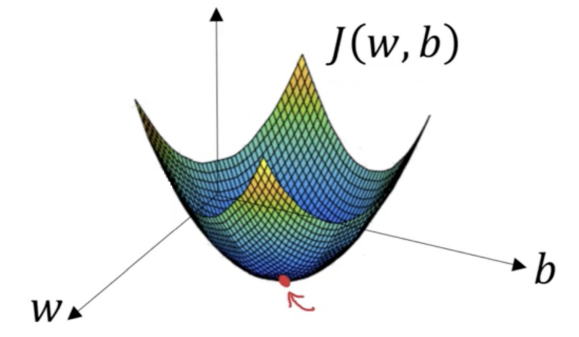
\includegraphics[width=0.8\textwidth]{images/desarrollo/entrenamiento/gradient}
		\end{center}
		\begin{center}
		\caption{\small{Establecimiento de la Tasa de Aprendizaje}}
		{\small{\citep{gradientimg}}}
		\end{center}
		\vspace{-1.5em}
		\end{figure}
		

		La idea detrás del descenso de gradiente es disminuir de forma gradual, pero constante, el error de salida ajustando los pesos. Intuitivamente, se conoce que si un cambio en un peso aumentará (disminuirá) el error, entonces queremos disminuir (aumentar) ese peso. Matemáticamente, representa el cambio en el error dado un cambio de unidad en el peso:

		\begingroup\makeatletter\def\f@size{20.8}\check@mathfonts
		\begin{center}
		$ \frac{{\partial E}}{\partial w_{ij}}$
		\end{center}
		\begin{center}
		{\small{La derivada del error con respecto al peso}}
		\end{center}
		\endgroup
		
		Una vez que encontremos esta derivada, actualizamos el peso a través de lo siguiente:

		\begingroup\makeatletter\def\f@size{17.8}\check@mathfonts
		\begin{center}
		$  \triangle w_{ij} = -\eta\frac{{\partial E}}{\partial w_{ij}} $
		\end{center}
		\begin{center}
		{\small{Representación de la distancia por la dirección del cambio. $\eta$  es tasa de aprendizaje}}
		\end{center}
		\endgroup

		La tasa de Aprendizaje suele disminuir gradualmente durante las épocas de la fase de entrenamiento. Si actualizamos todos los pesos usando esta misma fórmula, esto equivale a moverse en la dirección de descenso más pronunciado a lo largo de la superficie de error, de ahí el nombre, descenso de gradiente.

		Se tienen diversos tipos, estos son:
		%con el objetivo principal de optimizar la funcion de error o pérdida de la red y por consecuente garantizar que el modelo neuronal pueda generalizar las clasificaciones a realizar. 
		\subsubsection{Gradiente Descendiente por Lotes(Batch Gradient Descent)}
		
			Calcula el error para cada ejemplo dentro del conjunto de datos de entrenamiento, pero el modelo se actualiza solo después de que se hayan evaluado todos los ejemplos de entrenamiento Todo este proceso es como un ciclo y se denomina época de entrenamiento.

		\subsubsection{Gradiente Descendiente Estocástico(Stochastic Gradient Descent-SGD)}

			Por el contrario, hace esto para cada ejemplo de entrenamiento dentro del conjunto de datos. Esto significa que actualiza los parámetros para cada ejemplo de entrenamiento, uno por uno. Esto puede hacer que el SGD sea más rápido que el Descenso de gradiente por lotes, dependiendo del problema. Una ventaja es que las actualizaciones frecuentes nos permiten tener una tasa de mejora bastante detallada. El hecho es que las actualizaciones frecuentes son más costosas desde el punto de vista computacional que el enfoque del BGD y La frecuencia de esas actualizaciones también puede generar gradientes ruidosos, lo que puede hacer que la tasa de error salte, en lugar de disminuir lentamente.

			El MOMENTUM es otro argumento en el optimizador SGD que podríamos ajustar para obtener una convergencia más rápida. Ayuda al vector de parámetros a aumentar la velocidad en cualquier dirección con un descenso constante del gradiente para evitar oscilaciones. Una elección típica de momento es entre 0.5 a 0.9.

		\subsubsection{Mini-batch Gradient Descent}

			Es el método de más usado, ya que es una combinación de los conceptos de SGD y Batch Gradient Descent. Simplemente divide el conjunto de datos de entrenamiento en pequeños lotes y realiza una actualización para cada uno de estos lotes. Por lo tanto, crea un equilibrio entre la robustez del descenso del gradiente estocástico y la eficiencia del descenso del gradiente discontinuo.





	\subsection{Tasa de Aprendizaje (Learning Rate)}
		Uno de los hiperparámetros clave durante el entrenamiento deuna red neuronal es la velocidad/tasa de aprendizaje para el descenso del gradiente.
		Este parámetro puede entenderse como el tamaño del paso en la optimización para minimizar la función de pérdida de la red, es decir, es un parámetro que determina cuánto influye un paso de actualización en el valor actual de los pesos, por ejemplo, el tamaño del paso en el que el gradiente cae en la dirección máxima de la pendiente, \citep {AdamImg}.

		Cuando la tasa de aprendizaje es demasiado pequeña, es necesario realizar muchas iteraciones de aprendizaje; pero cuando la tasa de aprendizaje es demasiado grande, el resultado se moverá hacia adelante y hacia atrás en ambos sentidos de los valores extremos(oscila), y no se podrá lograr la solución óptima.
		
		\begin{figure}[H]
		%\begin{center}
		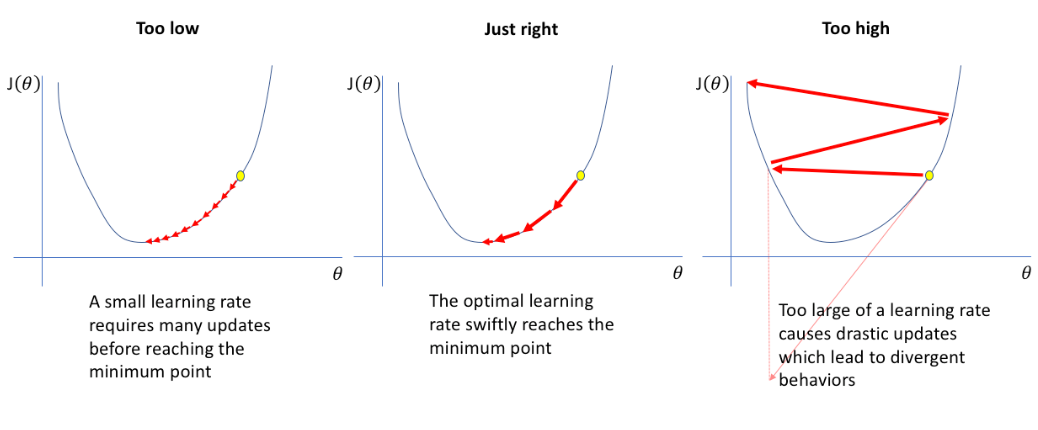
\includegraphics[width=1\textwidth]{images/desarrollo/entrenamiento/LR}
		%\end{center}
		\begin{center}
		\caption{\small{Establecimiento de la Tasa de Aprendizaje}}
		{\small{\citep {AdamImg}}}
		\end{center}
		\vspace{-1.5em}
		\end{figure}


		Debido a esto es que al entrenar redes neuronales profundas, a menudo es útil reducir la tasa de aprendizaje a medida que avanza el entrenamiento y no mantenerlo constante y asi evitar la divergencia(Punto apartir del cual la pérdida ya no se reduce y en lugar de eso comienza a incrementarse).


		\begin{figure}[H]
		%\begin{center}
		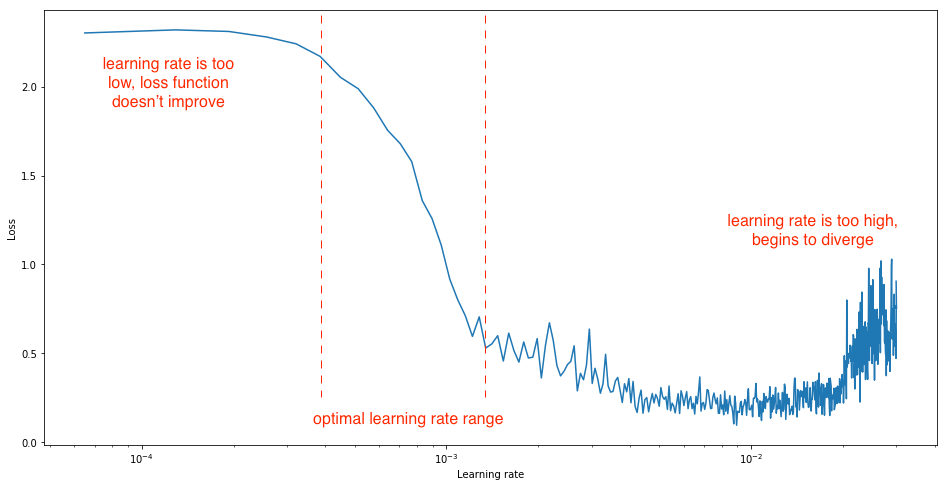
\includegraphics[width=1\textwidth]{images/desarrollo/entrenamiento/lr_finder}
		%\end{center}
		\begin{center}
		\caption{\small{Problemas con la Tasa de Aprendizaje}}
		{\small{\citep {AdamImg}}}
		\end{center}
		\vspace{-1.5em}
		\end{figure}

		Reduciendo lentamente la tasa de aprendizaje a lo largo del tiempo ayuda a acelerar el aprendizaje. Esto es lo que se conoce como tasa de decaimiento de aprendizaje{\bf(learning rate decay)}.
			\begin{figure}[H]
				\begin{center}
				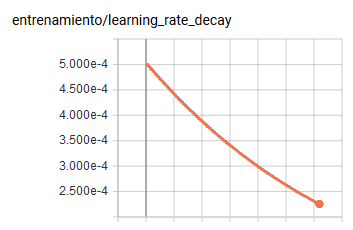
\includegraphics[width=0.7\textwidth]{images/desarrollo/entrenamiento/LR_decay} 
				\end{center}
				\begin{center}
				\caption{\small{Ejemplo de Tasa de decaimiento de aprendizaje por época  }}
				\vspace{-1em}
				{\small{\fontsize{10}{16.8}\selectfont {Fuente propia}}}
				\end{center}
				\vspace{-1.5em}
			\end{figure}
		Sin embargo, el optimizador Gradient Descent(en cualquiera de sus tipos) con una tasa de decaimiento de aprendizaje, no es usado a menudo para entrenar redes neuronales profundas ya que genera un desafío el determinar los hiperparámetros que deben definirse de antemano y dependen en gran medida del tipo de modelo y problema. Además de que la misma tasa de aprendizaje se aplica a todas las actualizaciones de los parámetros. Por lo que opta en usar optimizadores más avanzados que tienen una tasa de convergencia más rápida y adaptable a diversas situaciones. Proporcionan una alternativa a los clásicos y son conocidos como optimizadores de descenso de gradiente de segundo orden; algunos de ellos son: Adagrad, Adadelta, RMSprop, Adam. 

		%AdaGrad or adaptive gradient allows the learning rate to adapt based on parameters. It performs larger updates for infrequent parameters and smaller updates for frequent one. Because of this it is well suited for sparse data (NLP or image recognition). Another advantage is that it basically illiminates the need to tune the learning rate. Each parameter has its own learning rate and due to the peculiarities of the algorithm the learning rate is monotonically decreasing. This causes the biggest problem: at some point of time the learning rate is so small that the system stops learning.AdaDelta resolves the problem of monotonically decreasing learning rate in AdaGrad. In AdaGrad the learning rate was calculated approximately as one divided by the sum of square roots. At each stage you add another square root to the sum, which causes denominator to constantly decrease. In AdaDelta instead of summing all past square roots it uses sliding window which allows the sum to decrease. RMSprop is very similar to AdaDelta. Adam or adaptive momentum is an algorithm similar to AdaDelta. But in addition to storing learning rates for each of the parameters it also stores momentum changes for each of them separately

		En esta investigación se usaran los métodos de Descenso de Gradiente Mini-batch y optimzador Adam, conjuntamente con una tasa de decaimiento de aprendizaje.

	\subsection{Optimizador ADAM}
	
		El método calcula las tasas de aprendizaje individuales de manera adaptativa para diferentes parámetros a partir de las estimaciones de los primeros y segundos momentos de los gradientes; el nombre Adam deriva de Estimación del Momento Adaptativo \citep {Adam},

		Permite que la tasa de aprendizaje se adapte según los parámetros. Realiza actualizaciones más grandes para parámetros infrecuentes y actualizaciones más pequeñas para los frecuentes. Debido a esto, es adecuado para datos dispersos (NLP o reconocimiento de imágenes). Otra ventaja es que básicamente simplifica la necesidad de ajustar la tasa de aprendizaje. Cada parámetro tiene su propia tasa de aprendizaje, sin embargo, la tasa de aprendizaje no disminuye monótonamente. Además de almacenar las tasas de aprendizaje para cada uno de los parámetros, también almacena los cambios de momento para cada uno de ellos por separado .

	\subsection{Validación Cruzada}
	
		Para el entrenamiento, el conjunto de datos se divide en un subconjunto de entrenamiento y otro para validación. En esta investigación se dividirá el 75\% para entrenamiento y 75\% para validación, {\citep {Elkan12evaluatingclassifiers}}. La división en subgrupos de entrenamiento y validación generalmente se realiza de manera aleatoria, para garantizar que ambos subconjuntos sean muestras aleatorias de la misma distribución. Puede ser razonable realizar un muestreo estratificado, lo que significa asegurar que cada clase esté presente en la misma proporción en los subconjuntos de entrenamiento y prueba. En esta investigación se trabajará con 2 tipos de muestreos (balanceado/estratificado y no balanceado)

		Se utiliza el subconjunto de validación para evaluar el desempeño de diferentes arquitecturas del modelo (diferentes topologías), para luego escoger una de ellas. Este subconjunto(de validación) se usa para verificar si el error está dentro de algún rango y no se usa directamente para ajustar los pesos, por el contrario \textbf{se usa para indique el número óptimo de neuronas ocultas o determina el punto de parada para el entrenamiento}.  Por lo tanto, el modelo es entrenado sobre el conjunto de entrenamiento completo y la capacidad de generalización es medida en el conjunto de validación. 

		La validación cruzada o cross-validation es una técnica utilizada para evaluar los esultados de un análisis estadístico y garantizar que son independientes de la partición entre datos de entrenamiento y validación, \citep{moore2001cross}. En problemas de clasificación, debido a que los datos se dividen en clases finitas, es natural pensar que la categoría al cual pertenece cierto resultado se dará a través de probabilidades En probabilidad, la entropía cruzada es la distancia entre las dos distribuciones de probabilidad y se usa generalmente como la función de pérdida. Es por ello que el resultado de la validación cruzada representa la pérdida de la entropía del conjunto de datos. La entropía se suele utilizar en la teoría de la información para medir la pureza o impureza de un conjunto determinado. La pregunta a la que responde es: ¿Cuánto diferente esos elementos son entre sí?.  

			\begingroup\makeatletter\def\f@size{17.8}\check@mathfonts
			\begin{center}
			$H(p,q) = -\sum_{\forall x} p(x) log(q(x))$
			\end{center}
			\begin{center}
			{\small{Fórmula de entropía cruzada con dos distribuciones sobre la variable discreta $x$, donde $q(x)$ es la estimación para la clasificación verdadera $p(x)$}}
			\end{center}
			\endgroup		

		Para una red neuronal, normalmente verá la ecuación escrita en una forma donde $y$ es el vector de verdad y la variable $\hat{y}$ (o algún otro valor tomado directamente de la última salida de la capa) es la estimación, y se vería así para un solo ejemplo:
			
			\begingroup\makeatletter\def\f@size{17.8}\check@mathfonts
			\begin{center}
			$L = - \mathbf{y} \cdot log(\mathbf{\hat{y}})$
			\end{center}
			%\begin{center}
			%{\small{El valor es independiente de cómo la probabilidad restante se divide entre clases incorrectas}}
			%\end{center}
			\endgroup		
		
		A menudo esta ecuación es promediada sobre todos los ejemplos como una función de costo. No siempre se cumple estrictamente en las descripciones, pero generalmente una función de pérdida es de nivel inferior y describe cómo una sola instancia o componente determina un valor de error, mientras que una función de costo es de nivel superior y describe cómo se evalúa un sistema completo para la optimización. Una función de costo basada en pérdida de clasificación multiclase para un conjunto de datos de tamaño N podría verse así:
		
			\begingroup\makeatletter\def\f@size{17.8}\check@mathfonts
			\begin{center}
			$J = - \frac{1}{N}(\sum_{i=1}^{N} \mathbf{y_i} \cdot log(\mathbf{\hat{y}_i}))$
			\end{center}
			\begin{center}
			{\small{Cálculo de la función de costo en la validación de clasificación de datos}}
			\end{center}
			\endgroup		
	

		Es por ello que la la función de coste/pérdida dada por la validacion cruzada ayuda para decidir cuándo se debe terminar el entrenamiento de una red.\citep{AulaMLP}. Usualmente se utiliza el error cuadrático medio como función de pérdida para medir el rendimiento de un modelo de regresion. Sin embargo, en casos de clasificación, la función de costo de pérdida a través del cálculo de la entropía cruzada es preferible, ya que tiende a no causar saturación de las neuronas de salida, convirtiendo el aprendizaje más rápido,\citep{AulaDNN}.

		La pérdida de entropía cruzada aumenta a medida que la probabilidad prevista diverge de la clasificación real. Por lo tanto, un modelo casi perfecto tendría una pérdida de entropía cercana a cero, \citep{crossMSE}.
		


	\subsection{Función Softmax}
		Conocida tambien como función exponencial normalizada, es la funcion de activación utilizada en la última capa de una red neuronal. La salida de una red neuronal completamente conectada no es una distribución de probabilidad, sin embargo, el uso de esta función ayuda a obternela. Por lo que esta función permitirá estimar la probabilidad de que la imagen de entrada pertenezca a cada una de las clases al realizar una normalización con el objetivo que el valor de cada neurona esté limitado entre cero y uno y así permitir que el resultado de las neuronas de salida sumen a uno. 

			\begingroup\makeatletter\def\f@size{17.8}\check@mathfonts
			\begin{center}
			${\displaystyle P(y=j\mid \mathbf {x} )={\frac {e^{\mathbf {x} ^{\mathsf {T}}\mathbf {w} _{j}}}{\sum _{k=1}^{K}e^{\mathbf {x} ^{\mathsf {T}}\mathbf {w} _{k}}}}}$
			\end{center}
			\begin{center}
			{\small{Función Softmax}}
			\end{center}
			\endgroup
			
		Esto se puede ver como la composición de K funciones lineales ${x} \mapsto \mathbf {x} ^{\mathsf {T}}\mathbf {w} _{1},\ldots ,\mathbf {x} \mapsto \mathbf {x} ^{\mathsf {T}}\mathbf {w} _{K}$, donde ${\mathbf {x} ^{\mathsf {T}}\mathbf {w}}$ denota el producto interno de $x$(entrada) y $w$(peso).	La operación es equivalente a aplicar un operador lineal definido por $ w $ a vectores $ x $, transformando así la entrada original, probablemente altamente dimensional(reales arbitrarios), en vectores K-dimensional de valores reales en el rango [0, 1] que suman 1. \citep{Bishop}. 

		Esta función permite que al estar normalizadas las salidas de la segunda capa totalmente conectada, pueda ser aplicada la validación cruzada y conocer la pérdida de entropía.

	
	\subsection{Método de Regularización L2}
		En la regularización, lo que se hace normalmente es mantener el mismo número de funciones, pero se reduce la magnitud de los coeficientes.

		

		El método de Regularización L2 o también conocido como Regresión Lasso (Lasso Regression - Least Absolute Shrinkage and Selection Operator), trata de agregar un término adicional(lambda) a la función de pérdida, la cual penaliza parametrizaciones con pesos más elevados,\citep{AulaMLP}, es decir, reduce el coeficiente de la función menos importante a cero, eliminando así algunas características. Por lo tanto, esto funciona bien para la selección de funciones en caso de que tengamos una gran cantidad de funciones.

		Si $L(\theta, D)$ es la función de pérdida (en esta investigación - entropía cruzada), $\theta$ es el conjunto de parámetros libres y $D$ es un ejemplo de entrenamiento, entonces a la función de pérdida regularizada será:

			\begingroup\makeatletter\def\f@size{17.8}\check@mathfonts
			\begin{center}
			$E(\theta,D) =L(\theta,D) +\lambda R(\theta)$
			\end{center}
			\endgroup
		

		Donde $R(\theta)$ caracteriza la complejidad del modelo y $\lambda$ representa la proporción de la pérdida total del modelo, generalmente $\lambda$ estará cerca de 0 porque si $\lambda$ es demasiado grande, conducirá a un ajuste insuficiente(underfitting). Por otro lado, para evitar el exceso de ajuste(overfitting) cuando se tiene una gran cantidad de características en su conjunto de datos, no optimizamos directamente $L(\theta,D)$ (cross entropy), sino que optimizamos $L(\theta,D) +\lambda R(\theta)$

		Se usará una constante {\bf lambda($\lambda$) = 0.0001}, por defecto. La regularización de pérdida L2 solo debe incluir los pesos de las capas totalmente conectadas, y normalmente no incluye a los bias(sesgos). La intuición detrás de esto es que el bias contribuye al overfitting(sobreajuste), y no estaría agregando ningún nuevo grado de libertad al modelo.











	